\documentclass{article}

\usepackage[margin=1in]{geometry}
\usepackage{amsmath,amsthm,amssymb}
\usepackage{bbm,enumerate,mathtools}
\usepackage[hidelinks]{hyperref}
\usepackage{tikz}
\usetikzlibrary{shapes.geometric}

\newenvironment{problem}[2][Problem]{\begin{trivlist}
\item[\hskip \labelsep {\bfseries #1}\hskip \labelsep {\bfseries #2.}]}{\end{trivlist}}
\newenvironment{solution}[1][Solution.]{\begin{trivlist}
\item[\hskip \labelsep {\bfseries #1}]}{\end{trivlist}}
\newenvironment{problempart}[1]{\begin{trivlist}\item[\textbf{Part #1.}]}{\end{trivlist}}
\newcommand{\set}[1]{\{ #1 \}}
\newcommand{\ang}[1]{\langle #1 \rangle}
\begin{document}

\title{Combinatorics: Homework 12}
\author{Peter Kagey}

\maketitle

% -----------------------------------------------------
% First problem
% -----------------------------------------------------
\begin{problem}{1}
  Show that $R_2(3,4) = 9$.
\end{problem}

\begin{proof} $ $ \\
  $R_2(3,4) > 8$ because the coloring of $K_8$ in Figure 1 has no subgraphs
  $K_3$ which are colored blue (solid), because the only blue edges are of neighbors
  around the border or opposite vertices. The coloring has no subgraphs of $K_4$
  colored red (dashed) because no edges around the border are colored red, so a choice
  of $K_4$ must include ``every other'' vertex around the border, and the two
  choices are constructed so that either choice has two blue edges.
  \begin{figure}[h]
    \center
    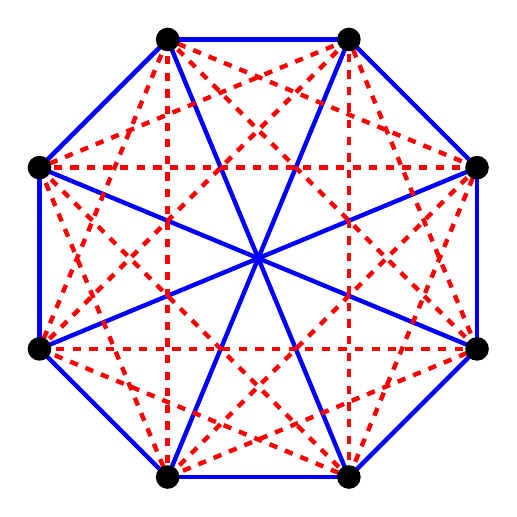
\begin{tikzpicture}
      \node[draw,minimum size=6cm,regular polygon,regular polygon sides=8] (a) {};

      \foreach \x/\y in {1/2,2/3,3/4,4/5,5/6,6/7,7/8,8/1,1/5,2/6,3/7,4/8} {
        \draw[ultra thick, blue] (a.corner \x)--(a.corner \y);
      }
      \foreach \x/\y in {
      1/3,2/4,3/5,4/6,5/7,6/8,7/1,8/2,
      1/4,2/5,3/6,4/7,5/8,6/1,7/2,8/3} {
        \draw[ultra thick, red, dashed] (a.corner \x)--(a.corner \y);
      }
      \foreach \x in {1,2,...,8} { \fill (a.corner \x) circle (0.15); }
    \end{tikzpicture}
    \caption{A $2$-coloring of $K_8$ which has no red $K_4$ subgraphs or blue
    $K_3$ subgraphs.}
  \end{figure}
  \\~\\
  Therefore it is sufficient to prove that $R_2(3,4) \leq 9$. We saw in class
  that $R_2(3,3) = 6$, and $R_2(2,4)$ = 4.
  Therefore take any vertex $v$ in $K_9$. Since $v$ has degree $8$, there are
  three cases to consider.
  \\~\\
  \textbf{Case 1.} Assume there are $5$ red edges and $3$ blue edges.
  Not all vertices can be in this case, because the sum of degrees
  must be even. If all nine vertices have three blue edges, then the sum of
  degrees in the blue subgraph is $27$, a contradiction. Thus,
  it is always possible to choose a vertex in one of the following two cases.
  \\~\\
  \textbf{Case 2.} Assume there are $6$ or more edges which are colored red.
  In this case, take six vertices which are connected to $v$ via a
  red edge, and look at the $K_6$ subgraph on these vertices. Because
  $R_2(3,3) = 6$ either $K_6$ has a blue $K_3$ (in which case $K_9$ does too,
  and we're done) or $K_6$ has a red $K_3$, in which case $K_3 \cup {v}$ is a
  complete graph on $4$ red vertices.
  \\~\\
  \textbf{Case 3.} Assume there are $4$ or more edges which are colored blue.
  In this case, take four vertices which are connected to $v$ via a
  blue edge, and look at the $K_4$ subgraph on these vertices. Because
  $R_2(4,2) = 4$ either $K_4$ is all red (and thus has a red $K_4$ subgraph,
  and we're done) or $K_4$ has a blue $K_2$ subgraph, in which case $K_2 \cup {v}$ is a
  complete graph on $3$ blue vertices.
\end{proof}
\pagebreak
% -----------------------------------------------------
% Second problem
% -----------------------------------------------------
\begin{problem}{2}
  Define $M_n$ recursively by \begin{align*}
    M_1 &= 3 \\
    M_m &= mM_{m-1} - m + 2.
  \end{align*} Show that \begin{enumerate}[(a)]
    \item $M_m = \lfloor m!\,e \rfloor + 1$
    \item If each edge on the complete graph $K_{M_m}$ is colored in one of $m$
    colors, then there exists a monochromatic triangle.
  \end{enumerate}
\end{problem}

\begin{solution} ~
  \begin{enumerate}[(a)]
    \item By induction, the base case $m=1$ is clear since
    $M_1 = \lfloor 1!\,e\rfloor + 1 = 2 + 1 = 3$.
    Thus the identity \begin{align*}
      \lfloor m!\,e \rfloor
      &= \left\lfloor \frac{m!}{0!} + \frac{m!}{1!} + \hdots + \frac{m!}{m!}
        + \frac{m!}{(m+1)!} + \hdots \right\rfloor \\
      &= \frac{m!}{0!} + \frac{m!}{1!} + \hdots + \frac{m!}{m!}.
    \end{align*} holds for all $m \geq 1$ since \[
      \frac{m!}{(m+1)!} + \frac{m!}{(m+2)!} + \hdots
      = \frac{1}{(m+1)} + \frac{1}{(m+1)(m+2)} + \hdots
      \leq e - 2
      < 1
    \]
    Therefore,
    \begin{align*}
      M_{m+1} &= (m+1)M_m - (m+1) + 2 \\
              &= (m+1)(\lfloor m!\,e \rfloor + 1) - (m+1) + 2 \\
              &= (m+1)\lfloor m!\,e \rfloor + 2 \\
              % &= (m+1)\left\lfloor \frac{m!}{0!} + \frac{m!}{1!} + \hdots + \frac{m!}{m!} + \hdots  \right\rfloor + 2 \\
              &= (m+1)\left( \frac{m!}{0!} + \frac{m!}{1!} + \hdots + \frac{m!}{m!} \right) + 2 \\
              &= \frac{(m+1)!}{0!} + \frac{(m+1)!}{1!} + \hdots + \frac{(m+1)!}{m!} + 2 \\
              &= \underbrace{
                \frac{(m+1)!}{0!}
                + \frac{(m+1)!}{1!} + \hdots
                + \frac{(m+1)!}{m!}
                + \frac{(m+1)!}{(m+1)!}
              }_{\lfloor (m+1)!\, e \rfloor}
              \underbrace{- \frac{(m+1)!}{(m+1)!}}_{-1} + 2 \\
              &= \lfloor (m+1)!\, e \rfloor + 1.
    \end{align*}
    \item By induction, where the base case $m=1$ is clear from a 1-coloring of
    $K_3$ being a monochromatic triangle.
    \\~\\
    A vertex $v$ in $K_{M_m}$ has degree \[
      \deg(v) = M_m - 1 = \lfloor m!\,e\rfloor = \frac{m!}{0!} + \frac{m!}{1!} + \hdots + \frac{m!}{m!}
    \], so by
    the pigeonhole principle, there are at least \begin{align*}
      \left\lceil \frac{\deg(v)}{m} \right\rceil
      &= \left\lceil
        \underbrace{
          \frac{(m-1)!}{0!} + \frac{(m-1)!}{1!} + \hdots + \frac{(m-1)!}{(m-1)!}
        }_{\lfloor (m-1)!\,e\rfloor}
        + \frac{(m-1)!}{m!}
      \right\rceil \\
      &= \lfloor (m-1)!\,e\rfloor + 1 \\
      &= M_{m-1}
    \end{align*} vertices with the same color, say, blue.
    Therefore, by the induction hypothesis, the subgraph on these $M_{m-1}$
    vertices either have a monochromatic triangle in the colors up to blue, or
    it has a blue edge, and this constructs a blue triangle.
  \end{enumerate}
\end{solution}
\pagebreak
% -----------------------------------------------------
% Third problem
% -----------------------------------------------------
\begin{problem}{3}
  Let $r \in \mathbb P$. Prove that any 2-coloring of the complete graph on
  $(r-1)^2 + 1$ vertices has either every red tree or every green tree in $r$
  vertices.
\end{problem}

\begin{proof} \text{} \\
  As we showed in class, for a particular tree $T$ on $g$ vertices, \[
    K_{(r-1)(g-1)+1}
  \] either has a red $K_r$ or a green $T$.
  \\~\\
  If $K_{(r-1)(g-1)+1}$ does not have
  a red $K_r$, it follows that it must have \textit{every} green $T$ on $g$
  vertices, since $T$ was arbitrary to begin with.
  \\~\\
  If $K_{(r-1)(g-1)+1}$ does have a red $K_r$, then any tree on $r$ vertices can
  be realized as a spanning tree on $K_r$, so $K_r$ (and thus $K_{(r-1)(b-1)+1}$)
  has every red tree on $r$ vertices.
\end{proof}
\end{document}
